\documentclass[12pt]{article}
\usepackage{hyperref}
\usepackage{listings}
\usepackage{biblatex}
\usepackage{tikz}
\usepackage{refstyle}
\usepackage{mathabx}
\usepackage{amssymb}
\usepackage{caption}
\usepackage{float}
\usepackage{graphicx}
\usepackage{graphics}
\usepackage{subfig}
\graphicspath{{/storage/self/primary/Download/latexnew/tables}}
\graphicspath{{/storage/self/primary/Download/latexnew/image}}
\begin{document}
\title{\textbf{PLATFORMIO}}
\date{}
\maketitle
\begin{enumerate}
    \item \textbf{Question(GATE-IN-2021-36):}Given below \figref{fig:1} is the diagram of a synchronous sequential circuit with one $J-K$ flip-flop and one $T$ flip-flop with their outputs denoted as A and B respectively,with$J_A = (A'+B'),K_A = (A+B)$,and $T_B = A.$


\begin{figure}[H]
        \centering
	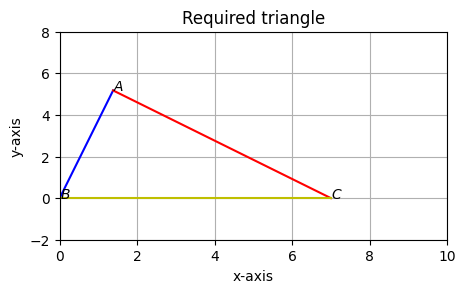
\includegraphics[width=\columnwidth]{image/2.png}
        \caption{}
        \label{fig:fig:1}
\end{figure}

   
    Starting from the initial state $(AB=00)$,the sequence of states $(AB)$ visited by the circuit is
    \begin{enumerate}
        \item $00\rightarrow01\rightarrow10\rightarrow11\rightarrow00 ...$
        \item $00\rightarrow10\rightarrow01\rightarrow11\rightarrow00 ...$
        \item $00\rightarrow10\rightarrow11\rightarrow01\rightarrow00 ...$
        \item $00\rightarrow01\rightarrow11\rightarrow00 ...$
    \end{enumerate}



    \textbf{Solution :}$J_A = A'+B'= (AB)'\\
    K_A = A+B;\\
    T_B = A.\\$
    As the given initial state is $AB = 00$.

		So,the required \underline{truth table} is as shown in \tabref{tab:1}.

   
    \begin{table}[!ht]
        \centering
	       \begin{tabular}{|c|c|c|}
    \hline
    \textbf{Input Parameters} &\textbf{Description} &\textbf{Value} \\
    \hline
     $\vec{O}$& Center(at origin)&$\vec{0}$\\
     \hline
 $r$ & Radius &1\\
 \hline
 $\theta$&-&$100\degree$\\
 \hline
 $\alpha$&-&$165.4\degree$\\
 \hline
 $\beta$&-&$5\degree$\\
 \hline
  \end{tabular}

        \caption{}
        \label{tab:tab:1}
    \end{table}
 $\therefore$ The sequence of the state $AB$ is $(b)00\rightarrow10\rightarrow01\rightarrow11\rightarrow00 ...$
\end{enumerate}


\end{document}
